\section{Bukin Function N.6}
\label{sec:app:test:bukin}

  The \emph{Bukin function N.6}, a two-dimensional benchmark problem, is
  renowned for its inherent complexity and frequent utilization in assessing
  optimization algorithms.
  Notable for a sharply defined, deep valley, the Bukin function N.6 presents 
  distinct hurdles for optimization techniques owing to its abrupt discontinuity
  and non-differentiability at \(x = 0\).

\begin{definition}[Bukin Function N.6]
  \label{def:app:test:bukin}
  The \emph{Bukin function N.6}, given by \(f: \mathbb{R}^2 \rightarrow 
  \mathbb{R}\), is mathematically represented as:

  \begin{equation}
    \label{eq:app:test:bukin}
    f(x,\, y) = 100 \sqrt{|y - 0.01x^2|} + 0.01 |x + 10|
  \end{equation}
  
  The decision variables, \(x,\, y \in \mathbb{R}\), typically have the prescribed
  domains: \(-15 \leq x \leq -5\) and \(-3 \leq y \leq 3\) respectively.
\end{definition}

The function attains its global minimum at \((x,\, y) = (-10, 1)\), yielding a 
value of zero.
The Bukin function N.6, due to its unique characteristics, offers 
a striking visualization.
A profound ridge, extending diagonally across the domain, forms a distinguishing
feature.
The contour and surface plots illustrating the Bukin function N.6 are presented 
in \vref{fig:app:test:bukin}.

\begin{figure}[ht!]
  \centering
  \begin{subfigure}[b]{0.4\textwidth}
    \centering
    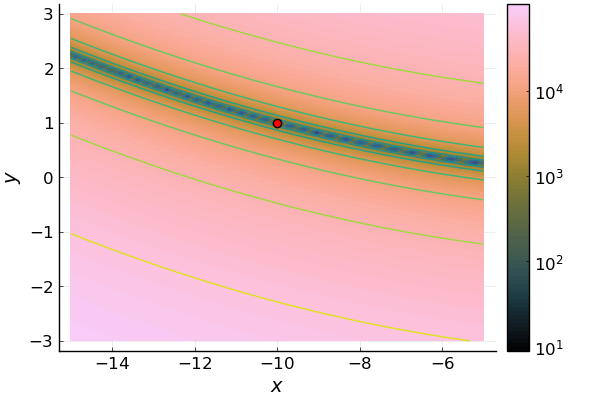
\includegraphics[width=\textwidth]{img/test_functions/bukin_contour.png}
    \caption{Contour plot of Bukin function N.6}
    \label{fig:app:test:bukin:contour}
  \end{subfigure}
  \hfill
  \begin{subfigure}[b]{0.4\textwidth}
    \centering
    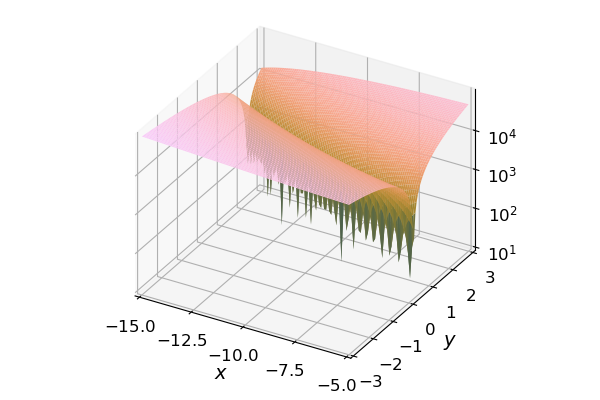
\includegraphics[width=\textwidth]{img/test_functions/bukin_surface.png}
    \caption{Surface plot of Bukin function N.6}
    \label{fig:app:test:bukin:surface}
  \end{subfigure}
  \caption{Contour and Surface Plots of Bukin Function N.6}
  \label{fig:app:test:bukin}
\end{figure}
